\chapter{Referencial Teórico}
\label{cap:referencial-reorico}

\section{O que é Machine Learning?}
\label{sec:oqueemachinelearning}

Embora a definição seja controversa, Tom M. Mitchell declara de forma plausível o que para ele é o principal objetivo de Machine Learning: "Machine Learning é o processo que faz com que um sistema melhore sua performance em determinada tarefa com base na experiência.". Podemos concluir através de sua definição que o processo de aprendizagem de um computador é semelhante ao que ocorre com nós seres humanos, onde onde em suma aprender é identificar padrões e reconhece-los quando vistos novamente.

\begin{alineas}
	\item Entrada de dados: são fatos tirados da memoria ou da observação;
	\item Abstração: transformar estes dados em algo mais objetivo e que faça sentido;
	\item Generalização: utiliza os dados abstraídos e para  identificar padrões e assim classifica-los;			
\end{alineas}

\begin{figure}[h!]
	\centering
	\Caption{\label{fig:processo-aprendizagem} Fluxo do processo de aprendizagem.}	
	\UECEfig{}{
		\fbox{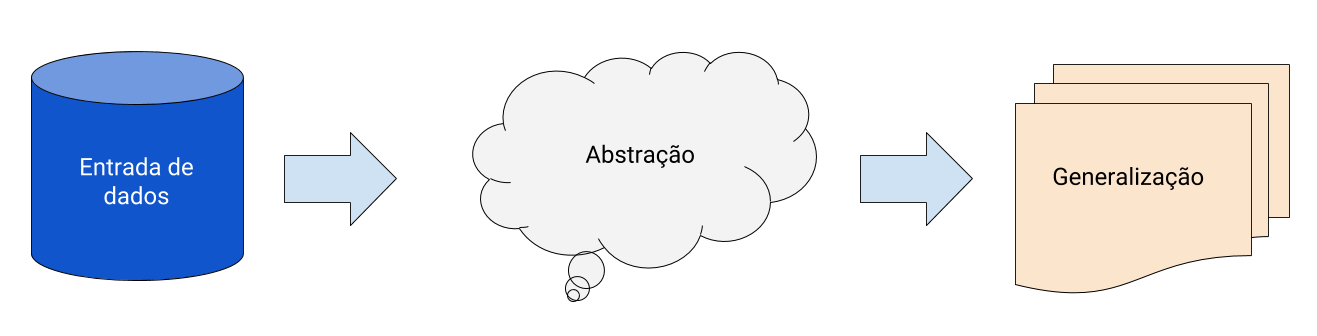
\includegraphics[width=15cm]{figuras/procc-learning}}
	}{
		\Fonte{Elaborado pelo autor}
	}	
\end{figure}

Todo este processo ocorre na ordem apresentada, pois o conceito de abstração e generalização estão muito próximos e tecnicamente um não faz sentido sem o outro. Os passos de abstração e generalização do processo de aprendizagem ocorrem subconscientemente em seres humanos, logo pode ser complexo representar este processo em linguagem computacional.


\subsection{Abstração e Representação de Dados}
\label{cap:abs-representacao-dados}

Durante a abstração os dados de entradas, são preparados para que possuam algum sentido em um contexto.
Para ilustrar este processo, lembre de quando aprendeu a executar operações de soma e subtração, que sua professora apresentou o exemplo:

\begin{figure}[h!]
	\centering
	\Caption{\label{fig:exemplo-aprendizagem} Uma maçã mais outra maçã é igual à duas maçãs.}	
	\UECEfig{}{
		\fbox{
\includegraphics[width=15cm]{figuras/exemplo_soma_maca}}
	}{
		\Fonte{Elaborado pelo autor}
	}	
\end{figure}

Você deixou de lado todas as propriedades da maçã como ser uma fruta, ter a cor vermelha  ou possuir sementes, para um tipo de unidade , uma unidade de um tipo mais outra unidade do mesmo tipo é igual à duas unidades, ou seja para o contexto de soma não importa se é uma fruta ou a cor e sim a unidade.

\begin{figure}[h!]
	\centering
	\Caption{\label{fig:exemplo-aprendizagem} Exemplo soma com maçãs após o processo de abstração.}	
	\UECEfig{}{
		\fbox{
\includegraphics[width=15cm]{figuras/exemplo_soma_maca2}}
	}{
		\Fonte{Elaborado pelo autor}
	}	
\end{figure}